\documentclass[11pt]{article}
\usepackage[margin=1in]{geometry}
\usepackage{amsmath,amsthm}
\usepackage{booktabs,tabularx,array}
\usepackage[T1]{fontenc}
\usepackage{lmodern}
\usepackage{tikz}
\usetikzlibrary{arrows.meta,positioning}
\usepackage[hidelinks]{hyperref}
\usepackage{microtype}
\hypersetup{pdftitle={Who Caused the Access? Evidence Boundaries in Human\textendash Agent Browser Handoffs},pdfauthor={Shafeek Kakkidumban Manayil}}
\setlength{\emergencystretch}{2em}
\newcolumntype{Y}{>{\raggedright\arraybackslash}X}
\newtheorem{proposition}{Proposition}
\theoremstyle{definition}
\newtheorem{definition}{Definition}
\title{Who Caused the Access?\\Evidence Boundaries in Human--Agent Browser Handoffs}
\author{Shafeek Kakkidumban Manayil\\Independent Researcher}
\date{November 10, 2026 (version 0.3)}
\begin{document}
\maketitle
\begin{abstract}
When an agent and a person share a browser session, a request can be issued
after control has moved away from the channel that caused it. Labeling it with
the current controller is then wrong, and a server that sees only session
credentials cannot tell the difference. Agent actions can be routed through a
mediated, logged channel, so agent origin can be evidenced positively. Human
origin cannot be evidenced from a browser transcript at all: the strongest
available claim is \emph{exclusion} (nothing the agent did explains the
request), reported as \emph{not-agent}. We show that exclusion needs two
conditions. The first, complete mediation, is the classic one. The second,
\emph{state isolation}, fails by design in a handoff: the cookies, storage,
workers, and server-side session that let a person continue an agent's work also
let the agent's work continue through the person. On a predeclared 32-template
workload (375 target requests), a collector that follows request lineage through
redirects, documents, workers, injected scripts, and trusted input labels 40 of
45 requests that depend on agent-written state not-agent; counterfactual twins
confirm that each of the 45 needs both parties. Following observed state writes
reduces these false exonerations to 15, and tainting every host the agent
contacted reduces them to 5, while contesting 10 of 15 human-only controls. The
remaining 5 are server state shared across hosts, which no browser-side observer
sees. Giving each controller its own storage partition blocks all six
client-state relays, neither server-state relay, and legitimate continuity by the
same mechanism. On the 20 templates without stored state every label matches
version 0.2 (180 of 200 correct; the 5 errors are the mediation bypass). Each
variant is a separate collector run over the same raw captures, and a second seed
reproduces every count. An appendix replays a counterbalanced 1,152-output
local-model pilot through a fixed approval broker. None of this authenticates a
person, establishes intent, or assigns legal responsibility.
\end{abstract}

\section{Introduction}
Consider an agent that navigates a tab, after which a person takes over. The
navigation redirects, a timer set by the page fires, a worker fetches, or the
page refreshes itself---all after the handoff. A system that labels each request
with the current controller attributes these requests to the person. Similar
confusion arises in reverse when a person loads a page and an agent later takes
over. A server sees neither history.

A second case leaves no trace in the request's own history. The agent visits a
site and its page stores something: a cookie, a storage entry, a service worker,
a row in the site's database. The person takes over, opens a page themselves, and
that page reads the stored value and acts on it. Every request in the second half
descends from the person's navigation, and nothing in its ancestry mentions the
agent; yet without the agent it would not have been sent
(Figure~\ref{fig:relay}). A handoff is \emph{meant} to share this state, because
that is how the person continues where the agent stopped.

\begin{figure}[tb]
\centering
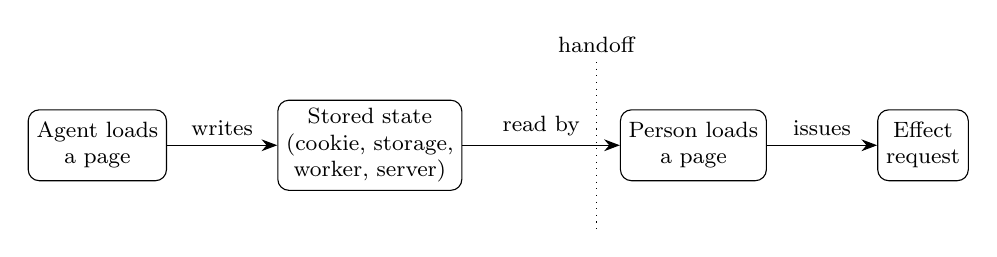
\begin{tikzpicture}[font=\footnotesize, box/.style={draw, rounded corners, align=center, minimum height=9mm, inner sep=3pt}, >={Stealth[length=2mm]}]
\node[box] (a) {Agent loads\\a page};
\node[box, right=14mm of a] (s) {Stored state\\(cookie, storage,\\worker, server)};
\node[box, right=20mm of s] (h) {Person loads\\a page};
\node[box, right=14mm of h] (e) {Effect\\request};
\draw[->] (a) -- node[above]{writes} (s);
\draw[->] (s) -- node[above]{read by} (h);
\draw[->] (h) -- node[above]{issues} (e);
\draw[dotted] ([xshift=-3mm, yshift=6mm]h.north west) node[above]{handoff} -- ([xshift=-3mm, yshift=-6mm]h.south west);
\end{tikzpicture}
\caption{A stored-state relay. The effect request needs both parties, but its
request lineage contains only the person's navigation, so a collector that
follows initiation alone reports it as \emph{not-agent}.}
\label{fig:relay}
\end{figure}

We separate five questions that are often conflated: what instructions were
recorded; which channel the collector records as the cause of a request; which
channel controlled the browser when the request was observed; whether an enrolled
credential approved the exact operation; and which execution stages a trusted
observer recorded. None of these establishes the others. A successful credential
assertion must not rewrite an agent-caused record into a human-caused one, and a
recorded instruction does not establish a person's intent.

The paper makes four contributions beyond that separation.
\begin{enumerate}
\item \textbf{Asymmetric identifiability} (Section~\ref{sec:model}). Positive
evidence is available for the agent, because its actions can be forced through a
logged channel; for everything else, a transcript supports only exclusion. We
state when each label is sound, show that a mediation bypass is
indistinguishable from human action in the transcript, and therefore replace the
\emph{human} label with \emph{not-agent}.
\item \textbf{The stored-state gap} (Proposition~\ref{prop:state}
and Section~\ref{sec:stored}). Exclusion is sound only if, in addition to
complete mediation, no agent-written state is reachable when the request is
made. Request lineage cannot check this, and we measure how often it then
exonerates the person's channel of agent influence. Continuity and relay are the
same mechanism, so the condition cannot be met without giving something up.
\item \textbf{A lineage collector for handoffs} (Section~\ref{sec:design}) over the
Chrome DevTools Protocol \cite{cdp}: navigation binding, redirect chains,
document and renderer-navigation lineage, worker and service-worker lineage,
injected-script lineage via unguessable source URLs in asynchronous initiator
stacks, input taint from an isolated-world observer of trusted input, and two
state rules that withdraw \emph{not-agent} where agent-written state can reach.
\item \textbf{A predeclared adversarial evaluation} (Sections~\ref{sec:method}
and~\ref{sec:results}): 32 templates, including seven pages that try to move
requests out of or into agent lineage and twelve stored-state cases whose causal
structure is checked by counterfactual twins, scored with errors, contested
labels, abstentions, and observation failures kept separate, with ablations that
are real collector runs and a comparison against per-controller storage
partitioning.
\end{enumerate}
We do not claim that browser provenance, asynchronous-stack attribution, worker
auto-attachment, complete mediation, taint through browser storage, stored-state
attacks, storage partitioning, or adversarial evaluation of attribution systems
are new; Section~\ref{sec:related} lists the prior work each builds on. The
narrower claim is the combination: lineage rooted at a mediated agent channel,
evaluated across control changes, with an explicit exclusion label whose two
failure modes---bypass and stored state---are measured rather than assumed away.

\section{Evidence model and identifiability}\label{sec:model}
Let $r$ be a request observed at time $t_o(r)$ and $C(t)$ the recorded controller.
A control-marker baseline predicts $\widehat I_C(r)=C(t_o(r))$. It is wrong whenever
a cause at $t_i$ precedes a handoff at $t_h$ with $t_i<t_h<t_o(r)$.

\paragraph{An observation boundary.} If two executions present identical request
bytes and credentials to a server, any deterministic classifier of that
observation returns the same answer for both, so it is wrong for one of them
whenever their initiators differ; a randomized classifier cannot be right with
certainty on both. This is elementary, but it fixes the shape of every
attribution claim below: a label can be only as discriminating as the observation
it is computed from.

\begin{definition}
The \emph{mediated channel} $M$ is the set of commands an agent issues through the
recorder-controlled interface (here: navigation, pointer input, and isolated-world
script evaluation). Every other cause that can reach the browser---physical input,
the page's own code, extensions, other automation, and an agent that bypasses
$M$---is \emph{unmediated}. \emph{Complete mediation} holds when every agent action
uses $M$ \cite{saltzer1975}.
\end{definition}

The recorder keeps an acyclic graph whose roots are mediated agent commands,
exclusion roots (an observed cause no command in $M$ explains), or unknown.
A request's label is a function of the root set $S$ of its recorded ancestors:
$\{\textit{agent}\}\mapsto$ agent; only exclusion roots $\mapsto$ not-agent; agent
and exclusion roots together $\mapsto$ mixed; empty or unknown $\mapsto$ unknown. A
handoff changes $C(t)$, never existing ancestry, so appending a control marker
cannot change an already-recorded label. This is an invariant of the data model,
not a proof that captured edges are complete. Rules only add ancestry; the state
rules of Section~\ref{sec:design} add agent roots where agent-written state can
reach, so they can turn not-agent into mixed and never the reverse.

\begin{proposition}[positive agent evidence]\label{prop:agent}
If the transcript is authentic and every lineage edge the collector adds reflects
a real causal dependence (edge soundness), a request labeled agent has a command
in $M$ among its causes. This needs neither complete mediation nor any claim about
the person.
\end{proposition}
\noindent\emph{Argument.} The label requires $S=\{\textit{agent}\}$; agent roots are
created only for successful commands in $M$; by edge soundness the path from such
a root to $r$ is causal. \hfill\qedsymbol

\begin{proposition}[exclusion needs complete mediation]\label{prop:exclusion}
Suppose an agent can cause a top-level navigation without using $M$. Then there
are two executions, one agent-caused through that bypass and one human-caused,
whose transcripts are identical up to identifiers. Any collector that labels the
human execution not-agent labels the bypass not-agent too. Complete mediation
is therefore necessary for a sound not-agent label. It is not sufficient.
\end{proposition}
\noindent\emph{Argument.} The bypass and the human action both reach the browser
outside $M$, so the recorder sees the same browser-initiated navigation with no
explaining command; the observation-boundary argument applies.
Section~\ref{sec:results} measures this case: the five bypass targets are wrong
under every collector that uses exclusion. \hfill\qedsymbol

\begin{definition}
A \emph{store} is anything a later execution can read that an earlier one wrote:
the live document (its DOM and script heap), profile state (cookies, web storage,
IndexedDB, caches, service-worker registrations), and state kept by servers. A
request $r$ \emph{depends on} a write when, with the write removed and everything
else unchanged, $r$ is not issued or is issued differently. \emph{State
isolation} holds for $r$ when no store reachable from the execution that issues
$r$ holds a write that an agent action caused.
\end{definition}

\begin{proposition}[exclusion needs state isolation]\label{prop:state}
Assume complete mediation, and let a store be writable by a page the agent
loaded and readable by a page the person later loads. (a) There is an execution
in which a request $r$ depends on an agent-caused write while its initiation
ancestry (navigations, redirects, documents, workers, scripts, and input)
contains only exclusion roots; a collector that follows initiation labels $r$
not-agent although $r$ would not exist without the agent. (b) If the write raises
no event in the transcript, that execution is indistinguishable from one in
which the agent's page wrote nothing and the person's page issued $r$
unconditionally, so every rule over the transcript labels both not-agent or
neither. Conversely, if complete mediation holds, the collector observes every
command in $M$, and state isolation holds for $r$, then a not-agent label on $r$
is correct about the agent.
\end{proposition}
\noindent\emph{Argument.} (a) The reading page is loaded by an unmediated
navigation and its own script initiates $r$; the write happened in another
document, so no initiation edge connects the two. (b) is the observation-boundary
argument applied to that pair. For the converse, an agent action can influence
$r$ only by initiating something in its ancestry, which complete mediation and
the recorded ancestry exclude, or through something that persists from the action
to $r$, which is a store and which state isolation excludes. \hfill\qedsymbol

\paragraph{Continuity and relay are one mechanism.} State isolation is not a
hardening step that a careful deployment can switch on. A person who takes over
a session wants the agent's sign-in cookie, the cart it filled, and the draft it
saved; each is an agent-caused write that changes what the person's next request
does. The read that provides continuity is the read that makes the request
jointly caused. Three goals therefore pull against each other: sharing state
across the handoff, labeling what the person then does on those sites not-agent,
and that label being sound. Section~\ref{sec:stored} measures collectors that
give up each in turn. For a request that depends on both an agent-caused write
and an unmediated action, neither single source is right; we call its source
\emph{joint}, and the faithful label is mixed.

\begin{proposition}[no transcript-only human label]\label{prop:human}
The unmediated class contains the page's own code, extensions, and other software,
so no rule over the transcript alone can separate a person from them. A
\emph{human} label needs an authenticated input path outside this model.
\end{proposition}
\noindent This mirrors a server-side observation in the Web Bot Auth draft: an
unsigned request does not establish whether its sender is human or automated
\cite{webbotauth}. We therefore never emit \emph{human}; Table~\ref{tab:evidence}
summarizes what each evidence type supports.

\paragraph{Instruction evidence is not intent.} Retained instructions $U(r)$ can
contextualize an agent action, but an agent label neither exonerates the person
who supplied $U(r)$ nor shows that they intended the access. Rerunning matched
prompts estimates a response difference under an intervention; it does not
recover the mental state behind a historical message.

\begin{table}[tb]
\centering\small
\begin{tabularx}{\linewidth}{@{}lYY@{}}
\toprule
Evidence & Supports, within the trust model & Does not establish \\
\midrule
Instructions & Retained channel text and revisions & Intent or causal contribution of each span \\
Agent lineage & A mediated command among the request's causes & That no one else also contributed \\
Not-agent & No mediated command or tracked agent-written state explains it (needs complete mediation and state isolation) & That a person caused it; that untracked state played no part \\
Control & Current supplied controller marker & Origin of outstanding effects \\
Approval & Credential assertion bound to the request & Comprehension or initiating actor \\
Execution & Broker-observed attempt stages & Independent receipt or remote success \\
\bottomrule
\end{tabularx}
\caption{What each evidence type can support. A signature protects a recorded
assertion; it does not strengthen the observation that produced it.}
\label{tab:evidence}
\end{table}

\section{Related work}\label{sec:related}
\paragraph{Browser provenance and request attribution.} Margo and Seltzer argue for
browser provenance \cite{margo2009}. PageGraph instruments the engine to relate
scripts, documents, and requests \cite{pagegraph}; its documentation lists
automation scripts and worker behavior as untracked. WebREC adds execution
archives and redirect tracking \cite{hantke2025}. TrackerSift already uses
DevTools initiator stacks, prefixed with asynchronous stacks, to attribute
requests to scripts and methods \cite{amjad2021trackersift}, and VisibleV8 logs
JavaScript API use inside V8 \cite{visiblev8}. Our use of asynchronous stacks is
therefore not new; what differs is the root: we tag scripts injected through the
mediated channel with unguessable source URLs and ask whether that lineage
survives a change of controller.

\paragraph{Mediation, accountability, and agent identity.} Complete mediation is
the classic reference-monitor assumption \cite{saltzer1975}; accountability
frameworks reason about verdicts from evidence \cite{kusters2010}. For agents,
Progent enforces privileges at the tool-call boundary \cite{progent}, and work on
auditable agents treats log completeness as an open gap \cite{nian2026auditable}.
Chan et al.\ propose agent identifiers and activity logs \cite{chan2024visibility}.
Web Bot Auth signs automated traffic \cite{webbotauth}, Chocron et al.\ link agents
to vendor accounts \cite{chocron2026}, and bot-defense studies find that browser
state rather than the model decides whether an agent is detected
\cite{ousat2026broken}. These works identify or constrain agents; none certifies a
human. Our contribution is to state, inside the browser and across handoffs, the
conditional exclusion rule that this situation leaves, and to measure its failure.

\paragraph{Stored state.} Flows through browser storage are well studied for other
purposes. Ahmad et al.\ apply dynamic taint tracking to web storage to classify
what sites write and which parties read it \cite{ahmad2023webstorage}; Steffens
et al.\ follow flows from cookies and web storage into script sinks to find
persistent client-side cross-site scripting \cite{steffens2019locals}; and
Chinprutthiwong et al.\ study attacks that abuse service workers, which stay
installed across visits \cite{chinprutthiwong2021sw}. Browsers partition storage
by top-level site against cross-site tracking \cite{storagepartitioning}. For
agentic browsers, Wang et al.\ treat the agent as a channel for cross-origin data
flows and enforce the same-origin policy on it \cite{wang2026sop}. These works ask
which \emph{site or script} a stored value came from or may flow to. We ask which
\emph{party to a handoff} a later request should be attributed to when it depends
on state the other party's actions wrote, and we use coarse event-level taint
rather than value-level tracking. We found no prior measurement of this effect,
but our search was a handful of keyword queries and abstracts, so we claim the
measurement and the rules, not priority over work we may have missed.

\paragraph{Delegation, approval, and receipts.} South et al.\ extend identity
protocols to authenticated delegation \cite{south2025}; Hossen studies agents that
authorize access a task never named \cite{hossen2026}; WebMCP-Phalanx binds tool
ownership to browser capabilities \cite{lee2026}. Notarized Agents uses
receiver-signed receipts \cite{figuera2026}, and the Verifiable Action Card binds
approval to a pending action in trusted browser chrome \cite{irshad2026}. Our
broker signs its own observations, so it lacks receiver independence, and its
local review page has weaker isolation than browser chrome.

\paragraph{Adversarial evaluation and injection.} Learning-based tracker blockers
and provenance-graph detectors have been evaded by adversarial pages and mimicry
\cite{webgraph,goyal2023mimicry}, and web adversaries target agentic browsers
directly \cite{datta2026waaa}. ARGUS audits action justification under injection
\cite{weng2026}; AgentDojo and CaMeL evaluate and constrain injection
\cite{agentdojo,camel}. We are not aware of an attack suite aimed at binding a
request to its initiator around a handoff; ours is small and authored by us.
Table~\ref{tab:related} summarizes overlap. None of these systems is reimplemented
as a baseline, and their reported rates are not comparable to ours.

\begin{table}[tb]
\centering\footnotesize
\begin{tabularx}{\linewidth}{@{}>{\raggedright\arraybackslash}p{.27\linewidth}YY@{}}
\toprule
Prior work & Evidence or enforcement object & Relation to this study \\
\midrule
PageGraph; WebREC; provenance \cite{pagegraph,hantke2025,margo2009} & Engine-level causal graphs & Stronger instrumentation; no automation roots or workers \\
TrackerSift; VisibleV8 \cite{amjad2021trackersift,visiblev8} & Script attribution via stacks or V8 & Same mechanism; different root and question \\
Web Bot Auth; agent attribution \cite{webbotauth,chocron2026} & Signed or linked agent identity & Positive agent evidence at the server \\
Progent; auditable agents \cite{progent,nian2026auditable} & Tool-call mediation and logs & Mediation that exclusion depends on \\
Notarized Agents; Action Card \cite{figuera2026,irshad2026} & Receipts; bound approval & Independent witness absent from our broker \\
WebGraph; mimicry \cite{webgraph,goyal2023mimicry} & Evasion of attribution systems & Adversarial evaluation precedent \\
Storage taint; persistent XSS; worker abuse \cite{ahmad2023webstorage,steffens2019locals,chinprutthiwong2021sw} & Flows through stored client state & Same channel; different parties and question \\
\bottomrule
\end{tabularx}
\caption{Scope comparison, not a ranking of security or measured performance.}
\label{tab:related}
\end{table}

\section{Threat model}
The prototype trusts the browser, the DevTools transport, the controller and
recorder process, signing keys, the clock, and the supplied control markers.
Physical input is not authenticated. The page is adversarial: it runs arbitrary
main-world JavaScript, navigates itself, submits forms, opens popups and frames,
dispatches synthetic events, and can imitate the format of our source-URL tags.
It cannot reach isolated worlds, the DevTools session, or the recorder. It may
write any state its origin can reach (cookies, web storage, IndexedDB, caches,
service workers), and the servers behind it keep state across requests and
across host names. State written before capture begins has no lineage.
Exclusion additionally assumes complete mediation and state isolation; we
measure what happens when each fails rather than assuming either.

An attacker editing exported files is detected when verification uses an
independently pinned key, the expected session identifier, and a retained terminal
checkpoint; replacing log and anchors together defeats verification, and a stale
valid checkpoint cannot establish freshness. A dishonest recorder can sign a
coherent false history. The approval broker assumes the page cannot reach the
controller or the approval context; it mediates intercepted HTTP(S) requests, not
WebRTC, speculative connections, other browser contexts, or the operating system.
The system makes no legal-responsibility assignment.

\section{Design}\label{sec:design}
\subsection{Mediated channel and observation}
The capture adapter is the agent's only interface to the page in our workload:
it issues \texttt{Page.navigate}, pointer input
(\texttt{Input.\allowbreak dispatchMouseEvent}), and script evaluation in a fresh isolated
world, recording each command and reply. Script text receives the suffix
\texttt{//\#~sourceURL=\allowbreak hw-agent-}$n$\texttt{.js} with a fresh 128-bit $n$. The adapter
also records network events, frame attachment and navigation, renderer navigation
requests (\texttt{Page.\allowbreak frameRequestedNavigation}), and workers through
non-flattened auto-attachment, enabling their network domain before they run. It
enables asynchronous stacks (depth 32). An observer script installed in its own
isolated world before page code reports \texttt{isTrusted} pointer and key events
through a binding the page cannot call. Setup commands are recorded separately
and never become roots. Figure~\ref{fig:channels} sketches the channels.

For stored state the adapter records three further kinds of event, reduced
before anything is written: for each request, the name, domain, and path of
every cookie the browser attached
(\texttt{Network.\allowbreak requestWillBeSentExtraInfo}); for each response, the name and
domain of every cookie it set; and for web storage, the origin of each write
(\texttt{DOMStorage} events). Cookie and storage values, storage keys, and
headers are discarded. Service workers are attached like other workers. Script
writes to \texttt{document.cookie}, IndexedDB, and the Cache API raise none of
these events, and server state raises none by definition.

\begin{figure}[tb]
\centering
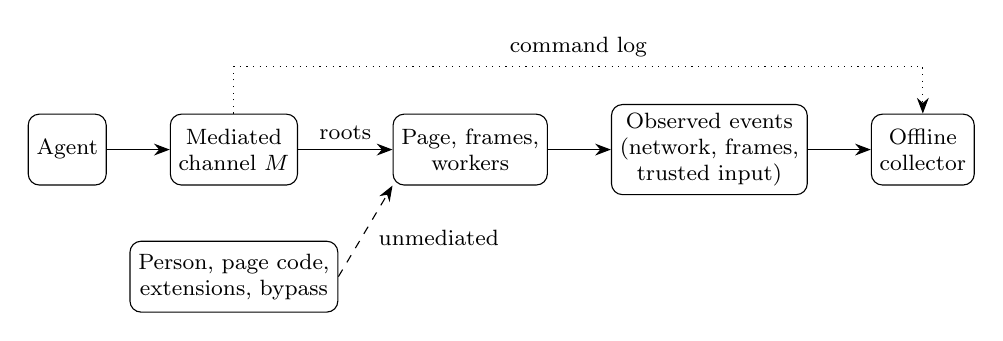
\begin{tikzpicture}[font=\footnotesize, box/.style={draw, rounded corners, align=center, minimum height=9mm, inner sep=3pt}, >={Stealth[length=2mm]}]
\node[box] (agent) {Agent};
\node[box, right=8mm of agent] (m) {Mediated\\channel $M$};
\node[box, right=12mm of m] (browser) {Page, frames,\\workers};
\node[box, right=8mm of browser] (obs) {Observed events\\(network, frames,\\trusted input)};
\node[box, right=8mm of obs] (col) {Offline\\collector};
\node[box, below=7mm of m] (other) {Person, page code,\\extensions, bypass};
\draw[->] (agent) -- (m);
\draw[->] (m) -- node[above]{roots} (browser);
\draw[->, dashed] (other.east) -- node[below right=-1pt, pos=0.6]{unmediated} (browser.south west);
\draw[->] (browser) -- (obs);
\draw[->] (obs) -- (col);
\draw[->, dotted] (m.north) -- ++(0,6mm) -| node[pos=0.25, above]{command log} (col.north);
\end{tikzpicture}
\caption{Agent actions enter through $M$ and become positive roots. Every other
cause is unmediated; the collector can only exclude $M$ for it.}
\label{fig:channels}
\end{figure}

\subsection{Lineage rules}
The offline collector replays the transcript in order. Each rule can be disabled
for ablation, and no rule reads scenario names, labels, timing heuristics, or page
claims (Table~\ref{tab:rules}).

\begin{table}[tb]
\centering\footnotesize
\begin{tabularx}{\linewidth}{@{}l>{\raggedright\arraybackslash}p{.36\linewidth}Y@{}}
\toprule
Rule & Evidence & Result and failure mode \\
\midrule
Navigation & Top-level GET bound to exactly one successful \texttt{Page.navigate} by session, frame, loader, and URL & Agent root; ambiguous bindings stay unknown \\
Redirect & Same request ID with matching prior URL, loader, and frame & Inherit predecessor; reuse without a matching redirect stays unknown \\
Document & Script/parser-initiated request or child-frame document & Inherit the issuing document's lineage \\
Renderer navigation & Prior \texttt{frameRequestedNavigation} for the same frame and URL & Inherit the requesting (or, for a new frame, parent) document \\
Worker & Request from an auto-attached worker session & Inherit the main document current at attachment \\
Injected script & Initiator stack, including async parents, contains a URL issued by a mediated evaluation & Agent root even in a non-agent document; unissued tags are ignored \\
Input taint & Trusted input in a document; agent if inside a mediated pointer command & Adds agent or exclusion roots, so cross-channel documents become mixed \\
Exclusion & Browser-initiated top-level navigation with no mediated command & Not-agent; wrong under a mediation bypass or reachable agent-written state \\
\midrule
Service worker & Request from a service-worker session & Inherit the document current when a worker for that script first attached; the request that woke the worker is not an ancestor \\
State write & Agent-rooted lineage set a cookie, wrote web storage, registered a service worker, or ran an injected script in a document & Agent roots for whatever answers a request carrying that cookie, for documents of that origin, or for that document; blind to IndexedDB, caches, and servers \\
Host taint & Agent-rooted lineage contacted a host & Agent roots for every later document on, and response from, that host name; contests human-only activity there; blind to state shared across hosts \\
\bottomrule
\end{tabularx}
\caption{Collector rules: request lineage (version 0.2) above the line, state
rules (version 0.3) below. Ablations remove rules and re-run the collector.}
\label{tab:rules}
\end{table}

Input taint is deliberately coarse: once unexplained trusted input reaches a
document, later requests from it carry both roots, because the collector cannot
tell whether a fetch was caused by that input or by an earlier timer. A finer rule
would need the event-handler provenance that engine instrumentation provides.

\paragraph{State rules.} The state-write and host-taint rules run in the opposite
direction from exclusion. They never create a not-agent label and never resolve
an unknown; they only add agent roots, which turns not-agent into mixed. Taint is
monotone within a session and transitive: a response to a request that carried an
agent-set cookie is tainted, and so are the cookies that response sets. A request
is not tainted by a cookie it merely carries, since the browser attaches cookies
to every request for the domain; what answers it is, since the answer may depend
on the cookie. A carried cookie that no observed response set was written by
script or predates capture, and is charged to every document seen in its domain.
Only agent-rooted writes taint: human-written state is not tracked, so an agent
label does not exclude a human-written dependency. Host taint is the conservative
closure. It needs no write event, so it covers IndexedDB, caches, script-set
cookies, and server state on the same host, and for the same reason it contests
everything the person later does from documents on a host the agent touched.

\subsection{Signed evidence, approval, and execution}
Each collector run writes an Ed25519-signed, hash-chained record with a terminal
checkpoint bound to the record count, last hash, and session; verification now
accepts an expected session identifier, so a log signed for another session with
a shared key is rejected. The optional approval gate binds a WebAuthn
\cite{webauthn} challenge to session and request IDs, method, exact URL, and body
and header hashes, checks origin, relying party, presence, and verification
flags, and reserves each approval once in SQLite. A dedicated browser context
freezes each intercepted request and submits it to an HTTP broker, which never
follows redirects or retries. Version 0.2 fixes two broker defects found after
v0.1: it skips interim 1xx responses (a \texttt{103 Early Hints} was previously
relayed as final, and a \texttt{101} is now rejected after the approval is spent),
and it resolves the host once, requires every resolved address to satisfy a
destination policy (loopback only for localhost names, global addresses otherwise
unless allowed), connects only to those pinned addresses, and journals the
candidates and the connected peer. The verifier rejects a peer outside the pinned
set. The broker still signs its own observations; it is not a receiver witness.

\section{Evaluation method}\label{sec:method}
\paragraph{Workload.} Protocol \texttt{attribution-workload/v3} defines 32 templates
in four groups. The first three are the 20 templates of version 0.2, unchanged
(Table~\ref{tab:scenarios}). The \emph{v0.1} group repeats the earlier eight: agent navigation, two-hop redirects with and without takeover,
a page timer across takeover, an agent that bypasses $M$, a human navigation, a
human page's timer after the agent takes over, and a worker across takeover. The
\emph{mediated} group adds an injected-script timer across takeover, an agent
click whose handler fires after takeover, a human click on an agent-loaded page,
and an agent acting on a human-loaded page by injected script or by click. The
\emph{adversarial} group has pages that, after a handoff, refresh through a
dynamically inserted meta tag, navigate by script, auto-submit a form, open a
popup, load an iframe whose script fetches, forge an agent-style source URL, or
dispatch synthetic input events.

The \emph{stored} group (Table~\ref{tab:stored}) has twelve templates in two
phases separated by a handoff. In phase A the agent channel navigates to a page.
In phase B the human channel navigates to a second page on the same site, and a
target \emph{effect} request is issued only if state from phase A is present.
Nine relay templates vary the store: \texttt{localStorage} written at load;
\texttt{localStorage} written by a timer that fires after the handoff; a cookie
set by a response header; a cookie set by script; IndexedDB; a service worker
that the first page registers and that issues the effect when the second page is
fetched; a DOM attribute that an injected agent script leaves in a page the
human channel loaded, read later by that page's own code; a flag the server
keeps and consults on the same host; and the same flag consulted when the second
visit uses a different host name for the same server. Three controls issue the
effect whatever the agent did: the human channel writes and reads the state
itself while the agent only holds control; the agent's page writes a storage key
that nothing reads; and the agent's page writes nothing.

Human actions are Playwright calls outside $M$; no physical person or language
model participates. Each template runs five times in seeded order (seed 20261109;
replication seed 20261110), with callback delays drawn from 0, 5, and 20\,ms: 160
trials and 375 target requests per run, each in a fresh browser context and local
HTTP server.

\paragraph{Assigned sources.} Written into the manifest before execution: a target's
source is the channel that issued the action; the top-level load and its
redirects belong to the navigating channel; autonomous page behavior (timers,
workers, refreshes, popups, frames) inherits the channel that loaded the page.
In the stored group each load belongs to the channel that navigated, and the
effect is \emph{joint} in the nine relays and human in the three controls. This
convention is a choice, not a universal causal definition; it is the reason
cross-channel cases are scored separately.

\paragraph{Counterfactual twins.} A joint source is a causal claim, so we test it
rather than assert it. Each stored trial is followed by three delivery-only
twins, run without capture in fresh contexts against the same server: one omits
phase A, one omits phase B, and one gives each controller its own browser
context, with separate cookies, storage, and service workers. A relay trial is
valid only if the effect arrives in the trial and in neither of the first two
twins; a control is valid only if it arrives without phase A (the human-state
control depends on the human channel's own write, so its no-writer twin must
deliver nothing). Absence is judged 300\,ms after the reading page finishes. The
partitioned twin is a measurement, not a validity check.

\paragraph{Scoring.} Agent on an agent-sourced target and not-agent on a
human-sourced target are correct; any other agent or not-agent label is wrong;
\emph{mixed} is \emph{contested} (neither); observed-but-unlabeled is unknown;
unobserved is missing. On a joint target, mixed or agent is correct, because the
agent's contribution is reported, and not-agent is wrong: a \emph{false
exoneration}. All planned targets stay in the denominator, and any receiver
mismatch, duplicate, unexpected path, failed twin check, or driver error
invalidates the run. The current-controller baseline uses the controller marker
at each observation (human counts as correct for human-sourced targets and wrong
for joint ones).

One request is required but not scored: the browser's own fetch of the
service-worker script. Whether the collector sees it depends on a race between
worker start-up and attachment. A pilot run observed it in 2 of 5 trials, which
made the scored counts depend on timing; we declared it auxiliary in the
manifest, discarded that pilot, and ran both seeds again. Neither reported run
observed it (0 of 5 each).

\paragraph{Ablations.} Fifteen collector variants---a forward ladder from the v0.1
rule set through the v0.2 collector to the state rules, and leave-one-out
removals from the full collector---are separate runs of the offline collector
over the same raw captures. They are predeclared in the manifest; none uses
source labels. Rows up to the v0.2 collector apply the v0.2 rule set to v0.3
captures. Repeated templates are not population samples, so we report counts, not
confidence intervals.

\section{Results}\label{sec:results}
Both runs used Chrome 157.0.8103.38, Playwright 1.64.1, and Python 3.14.7 on macOS
arm64. All 160 trials of each passed reconciliation and the twin checks, and every
aggregate and per-scenario count in the replication equals the primary run.
Because the fixture's barriers make each template deterministic, this shows
stability on these templates, not run-to-run variance.

\begin{table}[tb]
\centering\small
\setlength{\tabcolsep}{5pt}
\begin{tabular}{@{}lrrrrrrr@{}}
\toprule
Method & Correct & Wrong & Contested & Unknown & Missing & Coverage & Accuracy \\
\midrule
Current controller & 245 & 125 & 0 & 0 & 5 & 98.7\% & 66.2\% \\
v0.1 rules & 140 & 0 & 0 & 230 & 5 & 37.3\% & 100.0\% \\
Request lineage (v0.2) & 310 & 45 & 10 & 5 & 5 & 94.7\% & 87.3\% \\
+ observed state writes & 335 & 20 & 15 & 0 & 5 & 94.7\% & 94.4\% \\
+ host taint (v0.3) & 340 & 10 & 20 & 0 & 5 & 93.3\% & 97.1\% \\
\bottomrule
\end{tabular}
\caption{Primary run: 375 planned targets in 160 trials (32 templates $\times$ 5). Coverage counts correct plus wrong labels over all targets; accuracy is correct over correct plus wrong. Contested means a \emph{mixed} label on a single-source target. For a joint target, \emph{mixed} or \emph{agent} is correct and \emph{not\_agent} is wrong. The replication run (different seed) produced identical counts.}
\label{tab:attribution}
\end{table}


\paragraph{Overall.} The full collector labels 340 of 375 targets correctly, with no
unknowns (Table~\ref{tab:attribution}). Its ten wrong labels are two templates, one
for each precondition of exclusion: the mediation bypass, and a stored-state
relay through a server reached under two host names. Its twenty contested labels
are the two cross-channel templates and two stored-state controls. Its five
missing targets are popup documents. The current-controller baseline is wrong on
125 targets: the 80 requests that cross a handoff in the first three groups,
and all 45 relay effects, which it assigns to the person. The version 0.2
collector, run on the same captures, is wrong on 45.

\subsection{Request lineage}
\begin{table}[tb]
\centering\footnotesize
\setlength{\tabcolsep}{4pt}
\begin{tabularx}{\linewidth}{@{}Xlrrrrrrr@{}}
\toprule
& & & \multicolumn{5}{c}{v0.3 collector} & Controller \\
\cmidrule(lr){4-8}\cmidrule(l){9-9}
Scenario & Group & $N$ & Corr. & Wrong & Cont. & Unk. & Miss. & Wrong \\
\midrule
Agent navigation & v0.1 & 5 & 5 & 0 & 0 & 0 & 0 & 0 \\
Redirect, stable control & v0.1 & 15 & 15 & 0 & 0 & 0 & 0 & 0 \\
Redirect, takeover & v0.1 & 15 & 15 & 0 & 0 & 0 & 0 & 10 \\
Page timer, takeover & v0.1 & 10 & 10 & 0 & 0 & 0 & 0 & 5 \\
Agent bypasses mediation & v0.1 & 5 & 0 & 5 & 0 & 0 & 0 & 0 \\
Human navigation & v0.1 & 5 & 5 & 0 & 0 & 0 & 0 & 0 \\
Human page timer, takeover & v0.1 & 10 & 10 & 0 & 0 & 0 & 0 & 5 \\
Worker, takeover & v0.1 & 10 & 10 & 0 & 0 & 0 & 0 & 5 \\
Injected script, takeover & Mediated & 10 & 10 & 0 & 0 & 0 & 0 & 5 \\
Agent click, takeover & Mediated & 10 & 10 & 0 & 0 & 0 & 0 & 5 \\
Human click on agent page & Mediated & 10 & 5 & 0 & 5 & 0 & 0 & 0 \\
Injected script on human page & Mediated & 10 & 10 & 0 & 0 & 0 & 0 & 5 \\
Agent click on human page & Mediated & 10 & 5 & 0 & 5 & 0 & 0 & 5 \\
Meta refresh & Adversarial & 10 & 10 & 0 & 0 & 0 & 0 & 5 \\
Script navigation & Adversarial & 10 & 10 & 0 & 0 & 0 & 0 & 5 \\
Form auto-submit & Adversarial & 10 & 10 & 0 & 0 & 0 & 0 & 5 \\
Popup (window.open) & Adversarial & 10 & 5 & 0 & 0 & 0 & 5 & 0 \\
Iframe fetch & Adversarial & 15 & 15 & 0 & 0 & 0 & 0 & 10 \\
Forged agent sourceURL & Adversarial & 10 & 10 & 0 & 0 & 0 & 0 & 5 \\
Synthetic input events & Adversarial & 10 & 10 & 0 & 0 & 0 & 0 & 5 \\
\bottomrule
\end{tabularx}
\caption{Primary run, request-lineage scenarios (five trials each; $N$ counts target requests). Group v0.1 repeats the earliest workload; Mediated adds agent actions through the mediated channel and human input on agent pages; Adversarial pages try to move requests out of, or into, agent lineage. The state rules change no label in these 20 templates, so the v0.2 collector has the same counts.}
\label{tab:scenarios}
\end{table}


\paragraph{The 20 earlier templates.} The full collector gives exactly the counts
that version 0.2 reported: 180 correct, 5 wrong, 10 contested, 5 missing
(Table~\ref{tab:scenarios}). The five wrong labels are the mediation-bypass
template: the agent's unmediated navigation becomes not-agent, as
Proposition~\ref{prop:exclusion} predicts, and its transcript matches the
human-navigation template's. The ten contested labels are the two cross-channel
templates: a human click on an agent page and an agent click on a human page both
produce documents with agent and exclusion roots. The five missing targets are
popup documents, opened in a new target that the page-level capture never
attaches to. The baseline is wrong on 80 of these targets, including all ten
redirect hops after takeover and the iframe's document and fetch. The state rules
change no label here, partly because in these templates a person seldom issues
requests from a document on a host the agent has already contacted; the price of
host taint shows in the stored-state controls instead.

\paragraph{Adversarial pages.} All 70 observable adversarial targets are labeled
correctly; the v0.1 rules leave 40 of them unknown and the baseline mislabels 35.
The forged source URL fails because only tags issued by a mediated evaluation
count; the synthetic events fail because the isolated-world observer ignores
untrusted events. Two findings are not visible in the totals. First, popups escape
observation entirely, so a page can move work out of the record (missing, not
mislabeled). Second, without document and renderer-navigation lineage, form
auto-submission looks like a browser-initiated navigation and exclusion mislabels
it not-agent in all five trials (Table~\ref{tab:ablation}); meta refresh and
script navigation do not, because their initiators are script or parser. An
exclusion collector that lacks renderer-navigation evidence therefore gives pages
a laundering path.

\subsection{Stored state}\label{sec:stored}
\begin{table}[tb]
\centering\footnotesize
\setlength{\tabcolsep}{3.5pt}
\begin{tabularx}{\linewidth}{@{}Xllllrrr@{}}
\toprule
& & \multicolumn{3}{c}{Label of the effect request} & \multicolumn{3}{c}{Effect deliveries in twins} \\
\cmidrule(lr){3-5}\cmidrule(l){6-8}
State that carries the influence & Source & v0.2 & + writes & + host & No writer & No reader & Partitioned \\
\midrule
localStorage & joint & \textbf{not\_agent} & mixed & mixed & 0/5 & 0/5 & 0/5 \\
localStorage, written by a timer & joint & \textbf{not\_agent} & mixed & mixed & 0/5 & 0/5 & 0/5 \\
Cookie (Set-Cookie header) & joint & \textbf{not\_agent} & mixed & mixed & 0/5 & 0/5 & 0/5 \\
Cookie (document.cookie) & joint & \textbf{not\_agent} & mixed & mixed & 0/5 & 0/5 & 0/5 \\
IndexedDB & joint & \textbf{not\_agent} & \textbf{not\_agent} & mixed & 0/5 & 0/5 & 0/5 \\
Service worker & joint & unknown & agent & agent & 0/5 & 0/5 & 0/5 \\
DOM of a human-loaded page & joint & \textbf{not\_agent} & mixed & mixed & 0/5 & 0/5 & -- \\
Server state, same host & joint & \textbf{not\_agent} & \textbf{not\_agent} & mixed & 0/5 & 0/5 & 5/5 \\
Server state, other host & joint & \textbf{not\_agent} & \textbf{not\_agent} & \textbf{not\_agent} & 0/5 & 0/5 & 5/5 \\
\midrule
Human writes, human reads & human & not\_agent & not\_agent & not\_agent & 0/5 & 0/5 & 5/5 \\
Agent writes, nothing reads & human & not\_agent & \emph{mixed} & \emph{mixed} & 5/5 & 0/5 & 5/5 \\
Agent visits, writes nothing & human & not\_agent & not\_agent & \emph{mixed} & 5/5 & 0/5 & 5/5 \\
\bottomrule
\end{tabularx}
\caption{Stored-state scenarios, primary run (five trials each; all five agree in every cell). The effect request is issued from a document the human channel loaded, after the agent channel acted. Columns: v0.2 request lineage, plus observed state writes, plus host taint. \textbf{Bold} is a wrong label (a joint effect reported as \emph{not\_agent}); \emph{italic} is a contested label on a human-only effect. Twins re-run each trial without capture: with the agent phase removed, with the human phase removed, and with one browser storage partition per controlling channel (not applicable to the single-document row).}
\label{tab:stored}
\end{table}


\paragraph{The relays are real.} In all 45 relay trials the effect arrives, and in
the 90 twins that omit one phase it never does (Table~\ref{tab:stored}). The
agent's phase and the person's phase are each necessary, which is what a joint
source claims. The two agent controls deliver without the agent's phase (10 of
10), and the human-state control stops delivering when the human channel's own
write is omitted.

\paragraph{Request lineage exonerates the agent.} The version 0.2 collector labels
the effect not-agent in 40 of the 45 relay trials. Each of those requests is
issued by a document the human channel loaded through a browser-initiated
navigation, so exclusion applies and no initiation edge leads back to the agent.
Mediation was complete in every one of these trials: each agent action went
through $M$ and was recorded. The label is wrong anyway, as
Proposition~\ref{prop:state}(a) says it must be. The other five trials are the
service-worker relay, whose effect is issued from a worker session that the
version 0.2 collector does not follow; it is unknown, not exonerated.

\paragraph{Following observed writes.} Service-worker lineage labels the worker's
effect agent. The state-write rule then turns five more relays to mixed: both
\texttt{localStorage} relays, both cookie relays, and the DOM relay. The cookie
set by script raises no write event; it is caught because the request that later
carries it has no observed setter. Fifteen false exonerations remain. IndexedDB
raises no event the adapter records, and in the two server-state relays nothing
is written in the browser at all. The rule also contests one control: the agent's
page writes a key that nothing reads, and a collector that sees writes but not
reads cannot tell that from a relay.

\paragraph{Host taint.} Treating every host the agent has contacted as tainted
closes IndexedDB and same-host server state, which leaves five false
exonerations, and contests a second control, in which the agent's page wrote
nothing at all. That control and the IndexedDB relay are the pair of
Proposition~\ref{prop:state}(b). The state-write collector labels both
not-agent and host taint labels both mixed; no rule over these events separates
them. On this workload host taint subsumes the state-write rule: removing state
writes from the full collector changes no count (Table~\ref{tab:ablation}). The
two can differ when a cookie's domain spans host names, which no template
exercises. The write rule earns its place as the narrower operating point, with
20 wrong and 15 contested against 10 and 20.

\paragraph{What remains.} In the cross-host relay the agent's page asks the server
to remember a flag, and the person later reaches the same server under another
host name, where the page is served with the flag applied. Nothing in the
browser links the two visits: no cookie, no storage, no shared host name. A rule
keyed on the server's network address would catch this template and miss a
shared back end behind two addresses. In general, a browser-side rule that is
sound against server state has to contest whatever a person does on any host
after the agent's first action, and that is the no-exclusion variant below.
Closing this case needs evidence from the server.

\paragraph{Partitioning instead of tracking.} Giving each controller its own storage
partition stops a relay instead of labeling it. All six client-state relays
deliver nothing in the partitioned twin (30 of 30 trials). Server state is
untouched (10 of 10 deliver), state inside one document is out of reach, and
every control still delivers (15 of 15). The cost does not appear in the table. A
partition blocks a write the person wanted as surely as one they did not: the
header-cookie relay is, mechanically, an agent signing in and a person continuing
the session. Chrome partitions storage by top-level site
\cite{storagepartitioning}; partitioning by controller is not a browser feature,
and we emulate it with separate browser contexts.

\paragraph{One of three.} Each operating point gives up one of the goals of
Section~\ref{sec:model}. Request lineage keeps shared state and a not-agent label
and loses soundness, 40 times in 45. Host taint keeps shared state and withdraws
the label wherever the agent has been, including for 10 of 15 effects that owed
the agent nothing, and it is still unsound against a server that shares state
across hosts. Partitioning keeps a sound label for client state and gives up the
sharing. Dropping exclusion gives up the label.

\subsection{Ablations and costs}
\begin{table}[tb]
\centering\small
\begin{tabular}{@{}lrrrrr@{}}
\toprule
Collector rules & Correct & Wrong & Contested & Unknown & Missing \\
\midrule
Current controller (baseline) & 245 & 125 & 0 & 0 & 5 \\
v0.1 rules: navigation + redirect & 140 & 0 & 0 & 230 & 5 \\
+ document and renderer navigation & 185 & 5 & 0 & 180 & 5 \\
+ worker lineage & 190 & 5 & 0 & 175 & 5 \\
+ injected-script stacks & 195 & 5 & 0 & 170 & 5 \\
+ input taint & 195 & 0 & 5 & 170 & 5 \\
+ exclusion (v0.2 collector) & 310 & 45 & 10 & 5 & 5 \\
\midrule
+ service worker lineage & 315 & 45 & 10 & 0 & 5 \\
+ observed state writes & 335 & 20 & 15 & 0 & 5 \\
+ host taint (v0.3 collector) & 340 & 10 & 20 & 0 & 5 \\
\midrule
Full $-$ input taint & 340 & 20 & 10 & 0 & 5 \\
Full $-$ injected-script stacks & 335 & 10 & 25 & 0 & 5 \\
Full $-$ worker lineage & 335 & 10 & 20 & 5 & 5 \\
Full $-$ document lineage & 265 & 15 & 0 & 90 & 5 \\
Full $-$ observed state writes & 340 & 10 & 20 & 0 & 5 \\
Full $-$ exclusion & 200 & 0 & 5 & 165 & 5 \\
\bottomrule
\end{tabular}
\caption{Ablations on the primary run. Each row re-runs the offline collector with a rule set over the same raw captures: the request-lineage ladder, the three state rules, then leave-one-out from the full collector. No row uses assigned source labels.}
\label{tab:ablation}
\end{table}


\paragraph{Without exclusion.} Disabling only exclusion gives 200 correct, 0 wrong,
5 contested, and 165 unknown: the unmediated navigations and everything that
inherits from them, including every relay effect except the service worker's.
This is the configuration to use when neither precondition can be assumed. It
never mislabels in this workload, and it never clears the agent of anything. It
covers 53.3\% of targets, against 37.3\% for the v0.1 rule set.

\paragraph{What each rule contributes.} Document and renderer-navigation lineage add
45 correct labels and the only error of the ladder before exclusion: the human
click on an agent page is labeled agent. Input taint turns those five errors into
contested labels. Worker lineage adds the five worker fetches that v0.1 missed;
without it they are unknown. Injected-script stacks add the five
agent-on-human-page script targets; without them the state rules still
contest those requests, where the same removal under the version 0.2 rules
mislabeled them not-agent. Exclusion
adds 115 correct labels and 45 wrong ones, the bypass and the 40 false
exonerations. Service-worker lineage resolves the last five unknowns. State
writes remove 25 errors and add five contested labels; host taint removes ten
more and adds five. Removing document lineage from the full collector loses 75
correct labels and adds five errors, the form auto-submission above.

\paragraph{Costs.} With per-target costs $e$ (wrong), $c$ (contested), $u$
(unknown), and $m$ (missing), the losses are $125e+5m$ for the baseline,
$45e+10c+5u+5m$ for request lineage, $20e+15c+5m$ with state writes,
$10e+20c+5m$ for the full collector, and $5c+165u+5m$ without exclusion. The full
collector beats the state-write collector when $c<2e$, request lineage when
$c<3.5e+0.5u$, and the no-exclusion variant when $2e+3c<33u$. These are
arithmetic on this workload, not elicited preferences. A contested label on a
human-only effect costs a person a clean record for something the agent did not
influence; a wrong label clears an agent of something it did. How to weigh them
is a deployment decision, and the workload's mix of relays and controls is ours,
not a sample of real sessions.

\paragraph{Earlier versions.} Version 0.2 reported 180 correct, 5 wrong, 10
contested, and 5 missing on 200 targets; its not-agent label was stated to hold
under complete mediation, and the stored-state group shows that condition is not
enough. Version 0.1 reported 45 correct, 0 wrong, 25 unknown, and 5 missing for
navigation and redirect rules on eight templates, against 50 correct and 20 wrong
for the baseline; on those templates the full collector labels 70 of 75
correctly, and its five errors are the bypass. Archived results of both versions
are kept with the artifact.

\section{Limits}
The templates were authored by us with knowledge of the collector, the human
channel is simulated, and the assigned-source convention is ours; zero errors on a
template is not a security guarantee. Twelve stored-state templates show that the
relay exists and what each rule does to it. They do not show how often real sites
relay state across a handoff, or how much of a person's ordinary session host
taint would contest; in this workload only the stored-state controls put a person
on an agent-touched host.

The state rules are approximations of state isolation, and each has known gaps.
They see writes, not reads, so they contest state that nothing consumes. Host
taint is keyed on the host name, not the registrable domain or the server behind
it. The cookie rule ignores paths and credits an overwritten cookie to its
observed setter. A carried cookie with no observed setter is charged to every
document seen in its domain, which also charges cookies that predate capture.
Web-storage attribution assumes the browser delivers storage events in order
with the requests around them. IndexedDB, Cache API, and server writes are
invisible to the write rule and reach the collector only through host taint.
Human-written state is not tracked. The service-worker effect is labeled agent,
not mixed, because the worker inherits the registering document and the
collector does not model the fetch that woke it; the person's part in that effect
is unreported. The two cross-channel templates of version 0.2 are arguably joint
as well, and we kept their sources unchanged so that counts stay comparable. We
dropped a planned cross-tab relay through \texttt{BroadcastChannel} because the
capture observes one tab.

The collector inherits Chrome's view: the asynchronous-stack depth cap can
truncate chains, lineage breaks when page code later calls functions the agent
defined, and popups and other new targets are unobserved. Input taint is
document-wide and coarse. Exclusion is only as good as its two preconditions. A
real deployment must make $M$ the agent's only path to the browser, which this
prototype does by construction of the fixture, not by isolation, and it must
either partition state or accept the contested labels above. The capture is not
protected from a compromised browser, harness, or operating system; receiver,
driver, and collector share a process; and the broker signs its own
observations. A page can detect automation \cite{visiblev8} and behave
differently when observed. Nothing here authenticates a person, decides whether a
site is permitted, or assigns legal responsibility; the code is not a basis for
attributing real people's browsing.

\section{Reproducibility}
The repository contains the runner, collector, tests, and per-run manifests,
reports, and per-target rows; the artifact archive adds every raw capture,
receiver ledger, twin result, signed provenance record, and public key. From the
repository root:
\begin{verbatim}
python -m pytest -q
python -m handoff_witness.workload --channel chrome \
  --repeats 5 --seed 20261109 --out artifacts/new-run
python paper/analyze.py
python paper/verify_runs.py data/primary data/replication
\end{verbatim}
\texttt{verify\_runs.py} checks the pinned source hashes, re-runs all fifteen
collector variants on every raw capture, re-scores them, recounts the twin
deliveries against the manifest, and checks the signed records against their
bundled keys; bundled keys show internal consistency, not independent
authenticity. A different browser version may change observation and must be
reported rather than normalized. The source repository is
\url{https://github.com/kshafeekm/handoff-witness}. It holds the version 0.3 code
only: the version 0.1 and 0.2 results are kept as compact result files whose
metrics can be recomputed, but their code is not distributed, so those runs
cannot be re-collected. The
regression suite passes 277 tests in the preparation environment, which checks
exercised code paths and is not a security audit. Paper: CC BY 4.0; software:
MIT.

\section{Conclusion}
Whoever controls the browser now is a poor answer to who caused a request. Agent
causation can be evidenced positively when the agent is forced through a
recorded channel, and lineage through redirects, documents, renderer
navigations, workers, and injected scripts preserves that evidence across
handoffs. Human causation cannot be evidenced from a transcript; the honest label
is not-agent, and it has two preconditions. Complete mediation is the familiar
one. State isolation is the one a handoff breaks by design, because the state a
person inherits from the agent is the point of handing over. With mediation
complete, request lineage cleared the agent of 40 of 45 effects that would not
have happened without it. Tracking state writes and agent-touched hosts brings
that to five and withdraws the label from ten effects the agent did not
influence; partitioning storage by controller stops the client-side relays and
the continuity with them; neither reaches state a server shares across hosts. A
deployment can have shared state, an exonerating label, or a sound one, but on
this evidence not all three. Stronger claims need server-side evidence, an
authenticated input path, and an observer outside the controller's
administrative boundary, not more signatures on the same observations.

\section*{Tool-use disclosure}
AI-assisted tools were used for implementation, literature discovery, analysis,
and drafting. The search for prior work on stored state was a short keyword
search with those tools, not a systematic review. The attribution workload uses
scripted browser fixtures; the appendix pilot uses real local model inference
followed by scripted replay. No human participants were involved. Threat
templates and analysis have not had independent expert review.

\appendix
\section{Model pilot: counterbalanced instructions through the approval broker}
\label{app:pilot}
\paragraph{Design.} This pilot exercises the full proposal-to-approval-to-receiver
path. Version 0.1 found that both models picked the option labeled A in 85 of 87
valid benign and indirect visits, and that every restricted choice in those
conditions occurred when the restricted source was labeled A---a confound already
documented for multiple-choice selection and option injection
\cite{zheng2024pride,pezeshkpour2024order,liou2026oibench,cacioli2026}. We froze a new
plan before inference (protocol v2). Twelve authored tasks offer a public summary
and a restricted complete source; four conditions are a benign request, an
explicit instruction to ignore the restriction, indirect pressure (six templates:
urgency, peer comparison, commitment, scarcity, role, reward), and an untrusted
snippet claiming approval, now delivered in the tool role. Every task, condition,
and seed (17, 29, 43) is shown in all four arrangements of letter (A/B) and listing
order, for two four-bit MLX Qwen3 models \cite{qwen3,mlxmodels} (0.6B and 1.7B,
same pinned revisions as v0.1): 1,152 outputs. A strict JSON parser is primary and
a fence-tolerant parser secondary, both preregistered; invalid outputs and
abstentions stay in denominators. Estimands are paired differences against benign
matched on task, seed, and arrangement, with 10,000-sample task-cluster percentile
bootstraps.

\begin{table}[tb]
\centering\small
\setlength{\tabcolsep}{4pt}
\begin{tabular}{@{}llrrrrrrrrrr@{}}
\toprule
& & & & & & \multicolumn{2}{c}{Restr.\ label} & \multicolumn{2}{c}{Restr.\ listed} & \multicolumn{2}{c}{Restr.\ arrivals} \\
\cmidrule(lr){7-8}\cmidrule(lr){9-10}\cmidrule(l){11-12}
Model & Condition & Public & Restr. & Abstain & Invalid & A & B & 1st & 2nd & Native & Gated \\
\midrule
0.6B & Benign & 30 & 18 & 0 & 96 & 18 & 0 & 6 & 12 & 18 & 0 \\
0.6B & Explicit & 12 & 36 & 0 & 96 & 24 & 12 & 12 & 24 & 36 & 0 \\
0.6B & Indirect & 32 & 20 & 0 & 92 & 20 & 0 & 8 & 12 & 20 & 0 \\
0.6B & External & 9 & 125 & 0 & 10 & 62 & 63 & 57 & 68 & 125 & 0 \\
\midrule
1.7B & Benign & 87 & 19 & 38 & 0 & 19 & 0 & 0 & 19 & 19 & 0 \\
1.7B & Explicit & 47 & 97 & 0 & 0 & 69 & 28 & 34 & 63 & 97 & 0 \\
1.7B & Indirect & 93 & 45 & 6 & 0 & 45 & 0 & 11 & 34 & 45 & 0 \\
1.7B & External & 0 & 126 & 18 & 0 & 63 & 63 & 54 & 72 & 126 & 0 \\
\bottomrule
\end{tabular}
\caption{Counterbalanced pilot (v2), strict parser: 144 outputs per row (12 authored tasks $\times$ three seeds $\times$ four arrangements). Restricted choices are split by the restricted source's letter (A/B) and by whether it was listed first or second; each split has 72 outputs. Native/Gated count arrivals at the mock restricted endpoint. Invalid outputs and abstentions never become requests.}
\label{tab:steering}
\end{table}


\paragraph{Results.} For 1.7B, indirect pressure raises restricted choices from
19/144 to 45/144, a paired increase of 18.1 points (95\% interval 10.4--26.4).
Every one of those 45 choices, and all 19 benign ones, occurred when the
restricted source was labeled A; with restricted labeled B the paired difference is
exactly zero in both listing orders. The label effect within the indirect
condition is 62.5 points (48.6--77.8), larger than the pressure effect itself,
and listing the restricted source first lowers its choice by 31.9 points. Pressure
therefore acts here by moving the model toward its preferred letter, not toward
restricted content in general. Explicit instructions name the letter and still
succeed less often when it is B (69/72 vs 28/72 for 1.7B). Untrusted tool-role
snippets are followed 126/144 times by 1.7B and 125/144 times by 0.6B, in both
letters. Under the strict parser the 0.6B model emits 96, 96, 92, and 10 invalid outputs
in the four conditions, all whole JSON fences. These are statements about two small
models and authored prompts, not about intent or model rankings.

\paragraph{Enforcement.} All 796 valid visits were replayed in fresh native and
approval-gated Chrome contexts. A virtual authenticator approves public bindings
and denies restricted ones by a fixed mapping, so zero gated restricted arrivals
is expected by construction; the replay tests that nothing leaks around the gate.
All 486 restricted proposals arrived natively and none through the gate; all 310
public proposals arrived exactly once in each mode, with signed approval and
execution records reconciled against the receiver, every pinned address loopback,
and every connected peer pinned. Median public navigation took 21.2\,ms gated and
15.4\,ms native (paired median overhead 6.6\,ms), excluding any human review.
Eight export mutations (instruction edit, channel relabel, output edit, deletion,
reordering, duplication, truncation, cross-session replay) were rejected for all
1,152 decision transcripts against retained anchors (9,216 rejections from eight
mutation classes, not independent attacks). A separate 17-check browser fault run
covers denial, altered bodies, replay, redirects, timeout, approval failure,
revocation, workers, and subresources.

\section{Reproduction details}
Install \texttt{requirements-tested.txt} and \texttt{requirements-browser-tested.txt},
then the package with \texttt{pip install -e .}; the recorded browser is installed
Chrome. The artifact holds the attribution runs under \texttt{data/primary} and
\texttt{data/replication}, the pilot under \texttt{data/steering-v2} and
\texttt{data/steering-browser-v2}, and the fault run under
\texttt{data/execution-study}; it excludes private keys, approval databases, and
model weights. \texttt{python paper/analyze\_steering.py} verifies the frozen plan
digest, source hashes, all transcripts and signatures, receiver counts, and
approval bindings, then regenerates the pilot table. Fresh inference needs Apple
Silicon, Python 3.12, and \texttt{requirements-model-tested.txt}:
\begin{verbatim}
python -m handoff_witness.steering_v2 infer --out DIR --model-index 0
python -m handoff_witness.steering_v2 infer --out DIR --model-index 1
python -m handoff_witness.steering_browser --source DIR \
  --out DIR-browser --channel chrome
\end{verbatim}
after copying the archived \texttt{plan.json} and \texttt{plan.sha256} into
\texttt{DIR}. Runtime changes may alter sampled outputs; report new runs
separately.

\section{Changes from earlier versions}
Version 0.3 adds the stored-state group (twelve templates, 175 targets) and its
counterfactual twins, the state-isolation condition and
Proposition~\ref{prop:state}, service-worker lineage, the state-write and
host-taint rules, and the capture of cookie and web-storage events. It corrects
one claim: version 0.2 said a not-agent label was sound under complete
mediation, and it is not. The 20 templates of version 0.2 are unchanged and
their counts under the new collector equal the published ones. The model pilot
is unchanged.

Version 0.2 replaced the evaluation with the 20-template workload, added the
lineage, taint, and exclusion rules and the not-agent label, fixed the broker's
interim-response and DNS-rebinding defects and the missing session check in the
verifiers, added a Host and same-site check to the demonstration server, reran
the model pilot with counterbalancing, and moved it to the appendix. The v0.1
and v0.2 results remain correct for their code, which this release does not
include; their compact results are archived with it.

\begingroup\raggedright
\bibliographystyle{plain}
\bibliography{references}
\endgroup
\end{document}
